% Auto-generated by paper/figures/generate.py
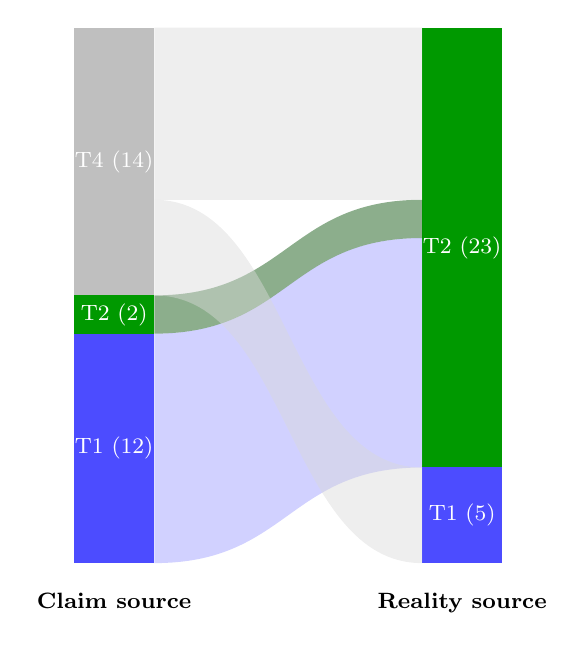
\begin{tikzpicture}[scale=0.85]
  \fill[blue!70] (0.0,0) rectangle (1.2,3.4285714285714284);\node[font=\footnotesize, white] at (0.6,1.7142857142857142) {T1 (12)};
  \fill[green!60!black] (0.0,3.4285714285714284) rectangle (1.2,4.0);\node[font=\footnotesize, white] at (0.6,3.714285714285714) {T2 (2)};
  \fill[gray!50] (0.0,4.0) rectangle (1.2,8.0);\node[font=\footnotesize, white] at (0.6,6.0) {T4 (14)};
  \node[font=\footnotesize\bfseries, anchor=north] at (0.6,-0.3) {Claim source};
  \fill[blue!70] (5.2,0) rectangle (6.4,1.4285714285714286);\node[font=\footnotesize, white] at (5.8,0.7142857142857143) {T1 (5)};
  \fill[green!60!black] (5.2,1.4285714285714286) rectangle (6.4,8.0);\node[font=\footnotesize, white] at (5.8,4.714285714285714) {T2 (23)};
  \node[font=\footnotesize\bfseries, anchor=north] at (5.8,-0.3) {Reality source};
  \fill[blue!40, opacity=0.45] (1.2,0.0) .. controls (3.2,0.0) and (3.2,1.4285714285714286) .. (5.2,1.4285714285714286) -- (5.2,4.857142857142857) .. controls (3.2,4.857142857142857) and (3.2,3.4285714285714284) .. (1.2,3.4285714285714284) -- cycle;
\fill[green!30!black, opacity=0.45] (1.2,3.4285714285714284) .. controls (3.2,3.4285714285714284) and (3.2,4.857142857142857) .. (5.2,4.857142857142857) -- (5.2,5.428571428571428) .. controls (3.2,5.428571428571428) and (3.2,4.0) .. (1.2,4.0) -- cycle;
\fill[gray!30, opacity=0.45] (1.2,4.0) .. controls (3.2,4.0) and (3.2,0.0) .. (5.2,0.0) -- (5.2,1.4285714285714286) .. controls (3.2,1.4285714285714286) and (3.2,5.428571428571429) .. (1.2,5.428571428571429) -- cycle;
\fill[gray!30, opacity=0.45] (1.2,5.428571428571429) .. controls (3.2,5.428571428571429) and (3.2,5.428571428571429) .. (5.2,5.428571428571429) -- (5.2,8.0) .. controls (3.2,8.0) and (3.2,8.0) .. (1.2,8.0) -- cycle;
\end{tikzpicture}
